\myheader{Guía 4: Transformada de Fourier}


\begin{ejercicio}
    Hallar, utilizando propiedades, la transformada de Fourier de las siguientes señales:
    
    \begin{align*}
        \inciso & x(t) = 
        \begin{cases} 
            1 + \cos(\pi t) & |t| \leq 1 \\
            0 & |t| > 1 
        \end{cases} & \hspace{\fill} 
        \inciso & x(t) = \frac{\sin(\pi t)}{\pi t} \frac{\sin(2\pi (t-1))}{\pi (t-1)} \\
        \inciso & x(t) = 
        \begin{cases} 
            e^{-t} & 0 \leq t < 1 \\
            0 & \mbox{en otro caso}
        \end{cases} & \hspace{\fill} 
        \inciso & \parbox{.3\textwidth}{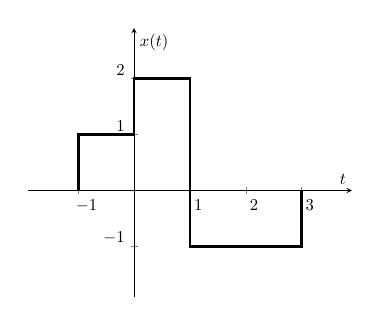
\begin{tikzpicture}[scale=0.6,transform shape]
    \begin{axis}[
    	axis y line=center,
    	axis x line=middle,
    	xlabel=$t$,ylabel=$x(t)$,
    	xmin=-1.9,xmax=3.9,
    	ymin=-1.9,ymax=2.9,
    	xticklabel style = {xshift=5},
    	yticklabel style = {yshift=5},
    	]
    	\addplot[
    	black,
    	ultra thick
    	] coordinates {
    	    (-1,0) (-1,1) (0,1) (0,2)
    	    (1,2) (1,-1) (3,-1) (3,0)
    	};
    \end{axis}
\end{tikzpicture}
} \\
        \inciso & \parbox{.3\textwidth}{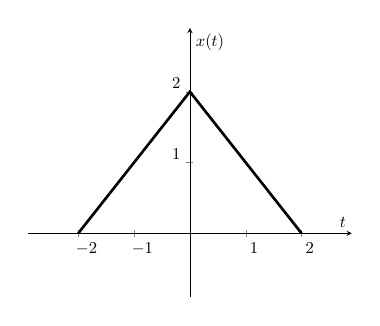
\begin{tikzpicture}[scale=0.6,transform shape]
    \begin{axis}[
    	axis y line=center,
    	axis x line=middle,
    	xlabel=$t$,ylabel=$x(t)$,
    	xmin=-2.9,xmax=2.9,
    	ymin=-0.9,ymax=2.9,
    	xticklabel style = {xshift=5},
    	yticklabel style = {yshift=5},
    	]
    	\addplot[
    	black,
    	ultra thick
    	] coordinates {
    	    (-2,0) (0,2) (2,0)
    	};
    \end{axis}
\end{tikzpicture}} & \hspace{\fill} 
        \inciso & \parbox{.3\textwidth}{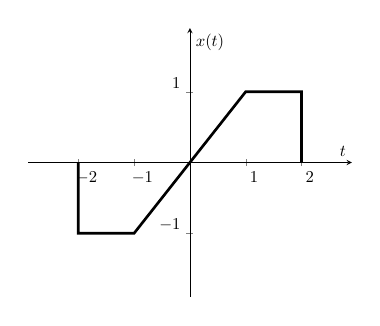
\begin{tikzpicture}[scale=0.6,transform shape]
    \begin{axis}[
    	axis y line=center,
    	axis x line=middle,
    	xlabel=$t$,ylabel=$x(t)$,
    	xmin=-2.9,xmax=2.9,
    	ymin=-1.9,ymax=1.9,
    	xticklabel style = {xshift=5},
    	yticklabel style = {yshift=5},
    	]
    	\addplot[
    	black,
    	ultra thick
    	] coordinates {
    	    (-2,0) (-2,-1) (-1,-1) (1,1) 
    	    (2,1) (2,0)
    	} ;
    \end{axis}
\end{tikzpicture}} \\
        \inciso & \parbox{.3\textwidth}{\begin{tikzpicture}[scale=0.6]
    \begin{axis}[
        x=.06\textwidth,y=0.1\textwidth,
    	axis y line=center,
    	axis x line=middle,
    	xlabel=$t$,ylabel=$x(t)$,
    	xmin=-7.9,xmax=7.5,
    	ymin=-0.3,ymax=2.3,
    	xticklabel style = {xshift=0},
    	yticklabel style = {yshift=5}
	]
	\diracdelta{-6}{2};
	\diracdelta{-5}{1};
	\diracdelta{-4}{2};
	\diracdelta{-3}{1};
	\diracdelta{-2}{2};
	\diracdelta{-1}{1};
	\diracdelta{0}{2};
	\diracdelta{1}{1};
	\diracdelta{2}{2};
	\diracdelta{3}{1};
	\diracdelta{4}{2};
	\diracdelta{5}{1};
	\node at (axis cs:6.5,1) {\Large $\cdots$} ;
	\node at (axis cs:-7,1) {\Large $\cdots$} ;
    \end{axis}
\end{tikzpicture}} & \hspace{\fill} & \\
    \end{align*}
    \end{ejercicio}
    
    \begin{ejercicio}
    Sea $x(t)$ la siguiente función:
    \begin{center}
        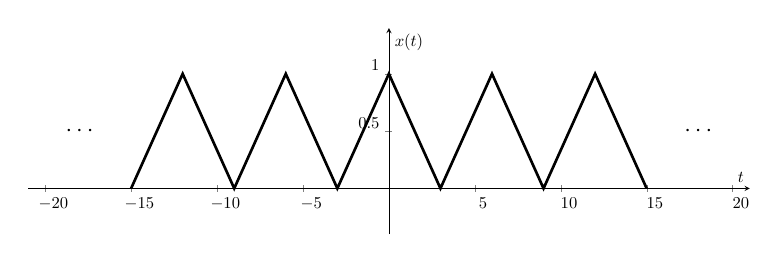
\begin{tikzpicture}[scale=0.6,transform shape]
    \begin{axis}[
        x=0.03\textwidth,y=0.2\textwidth,
    	axis y line=center,
    	axis x line=middle,
    	xlabel=$t$,ylabel=$x(t)$,
    	xmin=-21,xmax=21,
    	ymin=-0.4,ymax=1.4,
    	xticklabel style = {xshift=5},
    	yticklabel style = {yshift=5},
    	]
    	\addplot[
    	black,
    	ultra thick
    	] coordinates {
    	    (-15,0) (-12,1) 
    	    (-9,0) (-6,1)
    	    (-3,0) (0,1)
    	    (3,0) (6,1)
    	    (9,0) (12,1)
    	    (15,0)
    	};
    	\node at (18,0.5) {\Large $\cdots$} ;
    	\node at (-18,0.5) {\Large $\cdots$} ;
    \end{axis}
\end{tikzpicture}
    \end{center}
    
    \inciso Calcular la transformada de $x(t)$ utilizando la transformada $y(t) = \frac{\sin(\pi t)}{\pi t} \frac{\sin(2\pi (t-1))}{\pi (t-1)}$ calculada en el punto anterior. 
    
    \inciso ¿Qué relación existe entre la transformada de Fourier de una señal periódica y los coeficientes de su serie de Fourier? 
    
    \inciso ¿Qué característica distintiva tiene una Transformada de Fourier de una señal periódica?
    
    \end{ejercicio}
    
    
    \begin{ejercicio}
    Hallar, utilizando propiedades, la antitransformada de Fourier de las siguientes funciones:
    \begin{align*}
        \inciso & X(\omega) = \cos(4\omega + \pi/3) 
        \hspace*{10em} \inciso \hspace*{0.1em} X(\omega) = \frac{2\sin(3 (\omega-2\pi))}{\omega - 2\pi} \\
        \inciso & 
        X(\omega) \; \mathrm{tal\, que} \; |X(\omega)| = \begin{cases}
            |\omega| & \mbox{si } \omega \in [-1, 1) \\ 
            0 & \mathrm{en\, otro\, caso}
        \end{cases}
        \hspace*{1em} \mathrm{y} \hspace*{1em} \arg(X(\omega)) = -3\omega
    \end{align*}
    \end{ejercicio}
    
    \begin{ejercicio}
    Sea $X(\omega)$ la antitransformada de $x(t)$:
    \begin{center}
        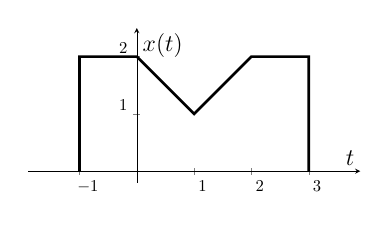
\begin{tikzpicture}[scale=0.6,transform shape]
    \begin{axis}[
        x=0.1\textwidth,y=0.1\textwidth,
    	axis y line=center,
    	axis x line=middle,
    	xlabel={\Large $t$},ylabel={\Large $x(t)$},
    	xmin=-1.9,xmax=3.9,
    	ymin=-0.2,ymax=2.5,
    	xtick distance=1,
    	ytick distance=1,
    	xticklabel style = {xshift=5},
    	yticklabel style = {yshift=5},
    	]
    	\addplot[
    	black,
    	ultra thick
    	] coordinates {
    	    (-1,0) (-1,2) (0,2) (1,1)
    	    (2,2) (3,2) (3,0)
    	};
    \end{axis}
\end{tikzpicture}

    \end{center}
    
    Hallar los siguientes valores sin obtener en forma explícita la función $X(\omega)$:
    \begin{align*}
        \inciso & \angle X(\omega) & \inciso & X(0) & \inciso & \int_{-\infty}^{\infty} X(\omega) d\omega \\[.5em]
        \inciso & \int_{-\infty}^{\infty} X(\omega) \frac{2\sin(\omega)}{\omega} e^{j2\omega} d\omega & \inciso & \int_{-\infty}^{\infty} |X(\omega)|^2 d\omega
    \end{align*}
    
    \end{ejercicio}
    
    \begin{ejercicio}
    Sea $x(t) = e^{-t} (u(t) - u(t-1))$. Graficar las siguientes funciones y hallar la transformada de Fourier de todas ellas:
    \begin{align*}
        \inciso & x_1 = x(-t) + x(t) & 
        \inciso & x_2 = -x(-t) + x(t) &
        \inciso & x_3 = x(t+1) + x(t) &
        \inciso & x_4 = t x(t)
    \end{align*}
\end{ejercicio}
    
\begin{ejercicio}
    Para cada una de las siguientes funciones
    \begin{align*}
        \inciso & \parbox{.5\textwidth}{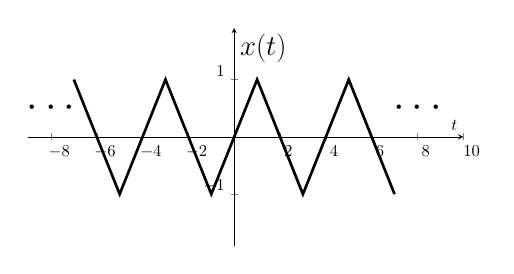
\begin{tikzpicture}[scale=0.6,transform shape]
    \begin{axis}[
        x=0.04\textwidth,y=0.1\textwidth,
    	axis y line=center,
    	axis x line=middle,
    	xlabel=$t$,ylabel={\LARGE $x(t)$},
    	xmin=-9,xmax=10,
    	ymin=-1.9,ymax=1.9,
    	xticklabel style = {xshift=5},
    	yticklabel style = {yshift=5},
    	]
    	\addplot[
    	black,
    	ultra thick
    	] coordinates {
    	    (-7,1) (-5,-1) 
    	    (-3,1) (-1,-1)
    	    (1,1) (3,-1)
    	    (5,1) (7,-1)
    	};
    	\node at (8,0.5) {\Huge $\cdots$} ;
    	\node at (-8,0.5) {\Huge $\cdots$} ;
    \end{axis}
\end{tikzpicture}} & \hspace{\fill} &
        \inciso & \parbox{.3\textwidth}{\begin{tikzpicture}[scale=0.6,transform shape]
    \begin{axis}[
    	axis y line=center,
    	axis x line=middle,
    	xlabel=$t$,ylabel=$x(t)$,
    	xmin=-2.9,xmax=2.9,
    	ymin=-0.9,ymax=2.9,
    	xticklabel style = {xshift=5},
    	yticklabel style = {yshift=5},
    	]
    	\diracdelta{1}{2};
    \end{axis}
\end{tikzpicture}} \\
        \inciso & \parbox{.5\textwidth}{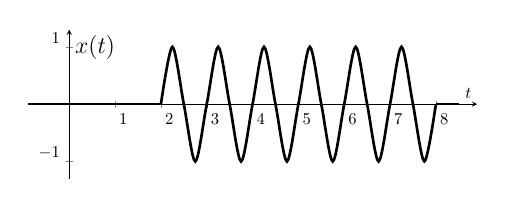
\begin{tikzpicture}[scale=0.6,transform shape]
    \begin{axis}[
        x=0.08\textwidth,y=0.1\textwidth,
    	axis y line=center,
    	axis x line=middle,
    	xlabel=$t$,ylabel={\Large $x(t)$},
    	xmin=-0.9,xmax=8.9,
    	ymin=-1.3,ymax=1.3,
    	xticklabel style = {xshift=5},
    	yticklabel style = {yshift=5},
    	]
    	\addplot [
    	black, ultra thick,
    	domain=2:8, smooth
    	] {sin(deg(2*pi*x))} ;
    	\addplot[
    	black, ultra thick
    	] coordinates {(-1,0) (2,0)} ;
    	\addplot[
    	black, ultra thick
    	] coordinates {(8,0) (8.5,0)} ;
    \end{axis}
\end{tikzpicture}} & \hspace{\fill} &
        \inciso & \parbox{.3\textwidth}{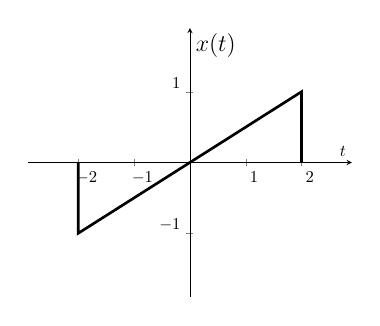
\begin{tikzpicture}[scale=0.6,transform shape]
    \begin{axis}[
    	axis y line=center,
    	axis x line=middle,
    	xlabel=$t$,ylabel={\Large $x(t)$},
    	xmin=-2.9,xmax=2.9,
    	ymin=-1.9,ymax=1.9,
    	xticklabel style = {xshift=5},
    	yticklabel style = {yshift=5},
    	]
    	\addplot[
    	black,
    	ultra thick
    	] coordinates {(-2,0) (-2,-1) (2,1) (2,0)} ;
    \end{axis}
\end{tikzpicture}} \\
        \inciso & \parbox{.5\textwidth}{\pgfmathdeclarefunction{ejcuatrotresa}{1}{%
  \pgfmathparse{#1^2 * exp(-abs(#1))}%
}

\begin{tikzpicture}[scale=0.6,transform shape]
    \begin{axis}[
        x=0.04\textwidth,y=0.2\textwidth,
    	axis y line=center,
    	axis x line=middle,
    	xlabel=$t$,ylabel={\Large $x(t)=t^2 e^{-|t|}$},
    	xmin=-8.9,xmax=8.9,
    	ymin=-.3,ymax=1.3,
    	xticklabel style = {xshift=5},
    	yticklabel style = {yshift=5},
    	samples=100
    	]
    	\addplot [
    	black, ultra thick,
    	domain=-10:10, smooth
    	] {ejcuatrotresa(x)} ;
    \end{axis}
\end{tikzpicture}} & \hspace{\fill} &
        \inciso & \parbox{.3\textwidth}{\pgfmathdeclarefunction{gauss}{3}{%
  \pgfmathparse{exp(-((#1-#2)^2)/(2*#3^2))}%
}

\begin{tikzpicture}[scale=0.6,transform shape]
    \begin{axis}[
        x=0.04\textwidth,y=0.2\textwidth,
    	axis y line=center,
    	axis x line=middle,
    	xlabel=$t$,ylabel={\Large $x(t)=e^{-t^2/2}$},
    	xmin=-4.9,xmax=4.9,
    	ymin=-.3,ymax=1.3,
    	xticklabel style = {xshift=5},
    	yticklabel style = {yshift=5},
    	]
    	\addplot [
    	black, ultra thick,
    	domain=-10:10, smooth, samples=100
    	] {gauss(x,0,1)} ;
    \end{axis}
\end{tikzpicture}} \\
    \end{align*}
    indicar si cumplen algunas de estas condiciones:
    \begin{align*}
        \subinciso & \Realpart{X(\omega)} = 0 &
        \subinciso & \Impart{X(\omega)} = 0 &
        \subinciso & \exists \alpha \in \mathbb{R} \; \mbox{tal que } e^{j\omega\alpha}X(\omega)\; \mbox{es una función real} \\
        \subinciso & \int_{-\infty}^{\infty} X(\omega) d\omega = 0 &
        \subinciso & \int_{-\infty}^{\infty} \omega X(\omega) d\omega = 0 &
        \subinciso & X(\omega)\; \mbox{es periódica}
    \end{align*}
\end{ejercicio}
    
\begin{ejercicio}
    Hallar y graficar la transformada de Fourier de tiempo discreto de las siguientes secuencias:
    \begin{align*}
        \inciso & x(n) = u(n) - u(n-20) &
        \inciso & x(n) = \delta(n) - \delta(n-1) \\
        \inciso & x(n) = \left( \frac{1}{2} \right)^{-n} u(-n-1) &
        \inciso & x(n) = \sin\left(\frac{\pi}{2} n \right) + \cos(n) 
    \end{align*}
\end{ejercicio}
        
\begin{ejercicio}
    Hallar la antitransformada de Fourier en tiempo discreto de las siguientes funciones:
    
    \inciso $X(e^{j\Omega}) = 1 + 3e^{-j2\Omega} - 4e^{-j10\Omega}$
    
    \inciso $X(e^{j\Omega}) = \sum_{k=-\infty}^{\infty} (-1)^k \delta(\Omega - \frac{\pi}{2}k)$
    
    \inciso $X(e^{j\Omega}) = \frac{e^{-j\Omega} - 1/5}{1-1/5 e^{-j\Omega}}$
    \end{ejercicio}
    
    \begin{ejercicio}
    Sea $X(e^{j\Omega})$ la antitransformada de Fourier de la secuencia $x(n)$:
    
    \begin{center}
    \parbox{.7\textwidth}{\begin{tikzpicture}[scale=0.6]
    \begin{axis}[
        x=.06\textwidth,y=0.1\textwidth,
    	axis y line=center,
    	axis x line=middle,
    	xlabel=$n$,ylabel=$x(n)$,
    	xmin=-7.9,xmax=11.9,
    	ymin=-1.3,ymax=2.3,
    	xticklabel style = {xshift=0},
    	yticklabel style = {yshift=5}
	]
	\discretedelta{-7}{0.1};
	\discretedelta{-6}{0.1};
	\discretedelta{-5}{0.1};
	\discretedelta{-4}{0.1};
	\discretedelta{-3}{-1};
	\discretedelta{-2}{0.1};
	\discretedelta{-1}{1};
	\discretedelta{0}{2};
	\discretedelta{1}{1};
	\discretedelta{2}{0.1};
	\discretedelta{3}{1};
	\discretedelta{4}{2};
	\discretedelta{5}{1};
	\discretedelta{6}{0.1};
	\discretedelta{7}{-1};
	\discretedelta{8}{0.1};
	\discretedelta{9}{0.1};
	\discretedelta{10}{0.1};
	\discretedelta{11}{0.1};
    \end{axis}
\end{tikzpicture}}
    \end{center}
    
    Hallar los siguientes valores sin obtener explícitamente la función $X(e^{j\Omega})$:
    \begin{align*}
    \inciso & X(0) & \inciso & \angle X(e^{j\Omega}) & \inciso & \int_{-\pi}^{\pi} X(e^{j\Omega}) d\Omega \\ 
    \inciso & X(e^{j\pi}) & \inciso & \int_{-\pi}^{\pi}  \left|\frac{X(e^{j\Omega})}{d\Omega}\right|^2 d\Omega &
    \end{align*}
\end{ejercicio}
    
    
\begin{ejercicio}
    Para cada una de las siguientes funciones
    \begin{align*}
        \inciso & \parbox{.3\textwidth}{\begin{tikzpicture}[scale=0.6,transform shape]
    \begin{axis}[
        x=0.04\textwidth,y=0.1\textwidth,
    	axis y line=center,
    	axis x line=middle,
    	xlabel=$n$,ylabel={\LARGE $x(n)$},
    	xmin=-4.9,xmax=8.9,
    	ymin=-0.3,ymax=2.9,
    	xticklabel style = {xshift=0},
    	yticklabel style = {yshift=5},
    	]
    	\discretedelta{-4}{0.1};
    	\discretedelta{-3}{0.1};
    	\discretedelta{-2}{0.1};
    	\discretedelta{-1}{0.5};
    	\discretedelta{0}{1};
    	\discretedelta{1}{1.5};
    	\discretedelta{2}{2};
    	\discretedelta{3}{1.5};
    	\discretedelta{4}{1};
    	\discretedelta{5}{0.5};
    	\discretedelta{6}{0.1};
    	\discretedelta{7}{0.1};
    	\discretedelta{8}{0.1};
    \end{axis}
\end{tikzpicture}} &
        \inciso & \parbox{.4\textwidth}{\begin{tikzpicture}[scale=0.6,transform shape]
    \begin{axis}[
        x=0.04\textwidth,y=0.1\textwidth,
    	axis y line=center,
    	axis x line=middle,
    	xlabel=$n$,ylabel={\LARGE $x(n)$},
    	xmin=-9.9,xmax=9.9,
    	ymin=-1.3,ymax=1.9,
    	xticklabel style = {xshift=0},
    	yticklabel style = {yshift=5},
    	]
    	\discretedelta{-8}{0.1};
    	\discretedelta{-7}{-1};
    	\discretedelta{-6}{0.1};
    	\discretedelta{-5}{1};
    	\discretedelta{-4}{0.1};
    	\discretedelta{-3}{-1};
    	\discretedelta{-2}{0.1};
    	\discretedelta{-1}{1};
    	\discretedelta{0}{0.1};
    	\discretedelta{1}{-1};
    	\discretedelta{2}{0.1};
    	\discretedelta{3}{1};
    	\discretedelta{4}{0.1};
    	\discretedelta{5}{-1};
    	\discretedelta{6}{0.1};
    	\discretedelta{7}{1};
    	\discretedelta{8}{0.1};
    	\node at (-9,0.5) {\Large $\cdots$};
    	\node at (9,0.5) {\Large $\cdots$};
    \end{axis}
\end{tikzpicture}} \\
        \inciso & \parbox{.3\textwidth}{\begin{tikzpicture}[scale=0.6,transform shape]
    \begin{axis}[
        x=0.03\textwidth,y=0.1\textwidth,
    	axis y line=center,
    	axis x line=middle,
    	xlabel=$n$,ylabel={\LARGE $x(n)$},
    	xmin=-9.9,xmax=9.9,
    	ymin=-1.3,ymax=2.9,
    	xticklabel style = {xshift=0},
    	yticklabel style = {yshift=5},
    	]
    	\discretedelta{-9}{0.1};
    	\discretedelta{-8}{0.1};
    	\discretedelta{-7}{0.1};
    	\discretedelta{-6}{0.1};
    	\discretedelta{-5}{0.1};
    	\discretedelta{-4}{-1};
    	\discretedelta{-3}{-1};
    	\discretedelta{-2}{0.1};
    	\discretedelta{-1}{0.1};
    	\discretedelta{0}{2};
    	\discretedelta{1}{-1};
    	\discretedelta{2}{0.1};
    	\discretedelta{3}{0.1};
    	\discretedelta{4}{1};
    	\discretedelta{5}{0.1};
    	\discretedelta{6}{0.1};
    	\discretedelta{7}{0.1};
    	\discretedelta{8}{0.1};
    \end{axis}
\end{tikzpicture}} &
        \inciso & \parbox{.4\textwidth}{\begin{tikzpicture}[scale=0.6,transform shape]
    \begin{axis}[
        x=0.04\textwidth,y=0.1\textwidth,
    	axis y line=center,
    	axis x line=middle,
    	xlabel=$n$,ylabel={\LARGE $x(n)$},
    	xmin=-9.9,xmax=9.9,
    	ymin=-1.3,ymax=2.9,
    	xticklabel style = {xshift=0},
    	yticklabel style = {yshift=5},
    	]
    	\discretedelta{-9}{0.1};
    	\discretedelta{-8}{0.1};
    	\discretedelta{-7}{0.1};
    	\discretedelta{-6}{2};
    	\discretedelta{-5}{0.1};
    	\discretedelta{-4}{-1};
    	\discretedelta{-3}{-1};
    	\discretedelta{-2}{0.1};
    	\discretedelta{-1}{1};
    	\discretedelta{0}{0.1};
    	\discretedelta{1}{1};
    	\discretedelta{2}{0.1};
    	\discretedelta{3}{-1};
    	\discretedelta{4}{-1};
    	\discretedelta{5}{0.1};
    	\discretedelta{6}{2};
    	\discretedelta{7}{0.1};
    	\discretedelta{8}{0.1};
    	\discretedelta{9}{0.1};
    \end{axis}
\end{tikzpicture}} 
    \end{align*}
    indicar si cumplen algunas de estas condiciones:
    \begin{align*}
        \subinciso & \Realpart{X(e^{j\Omega})} = 0 &
        \subinciso & \Impart{X(e^{j\Omega})} = 0 &
        \subinciso & \exists \alpha \in \mathbb{R}\; \mbox{tal que } e^{j\Omega\alpha}X(e^{j\Omega})\; \mbox{es una función real} \\
        \subinciso & \int_{-\pi}^{\pi} X(e^{j\Omega}) d\Omega = 0 &
        \subinciso & X(e^{j\Omega})\; \mbox{es periódica} &
        \subinciso & X(e^{j\Omega})|_{\Omega=0} = 0
    \end{align*}
\end{ejercicio}

\begin{ejercicio}
    Sea un sistema LTI discreto cuya respuesta al impulso es $h(n) = \left(\frac{1}{2}\right)^n u(n)$. Usando la transformada de Fourier de tiempo discreto hallar la salida $y(n)$ del sistema para las siguientes entradas:
    \begin{align*}
        \inciso & x(n) = \left(\frac{3}{4}\right)^n u(n) &
        \inciso & x(n) = (-1)^n u(n) \\
        \inciso & x(n) = A e^{j\frac{\pi}{2}n}, \; \mbox{con } A \in \mathbb{R} &
        \inciso & x(n) = 10 - 5 \sin\left(\frac{\pi}{2}n\right) + 20 \cos\left(\frac\pi n\right)
    \end{align*}
\end{ejercicio}

\begin{ejercicio}
    Utilizando la transformada de Fourier, decidir si existe un sistema LTI que cumpla con que, si $x(n)$ es la entrada, entonces $y(n)$ es la salida:
    
    \inciso $x(n)= e^{j\pi n/3}$ e $y(n) = \cos(\pi n/3)$

    \inciso $x(n) = \cos(\pi n/3)$ e $y(n) = \cos(\pi n/3) + \sqrt{3} \sin(\pi n/3)$
\end{ejercicio}

\begin{ejercicio}
    Sea la señal $x(t)$ cuya transformada de Fourier es $X(j\omega) = u(\omega - W_1) - u(\omega - W_2)$, con $W_1 < W_2$ y sea 
    \begin{equation*}
        y(t) = \frac{dx(t)}{dt} * x(t) + x(t)
    \end{equation*}
    Obtener $\int_{-\infty}^{\infty} |y(t-\alpha)|^2 dt$ donde $\alpha \in \R$.
\end{ejercicio}

\begin{ejercicio}
    Sea el siguiente sistema, donde $h_{pb}(n)$ es LTI:
    \begin{center}
    \parbox{.7\textwidth}{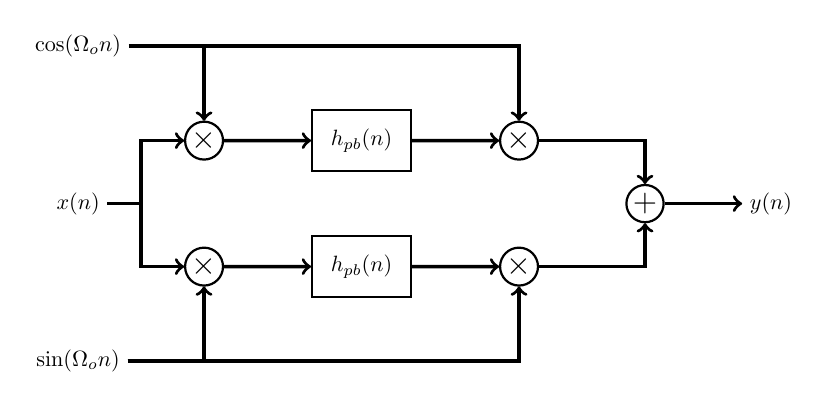
\begin{tikzpicture}[scale=0.8, transform shape]
    \node[circle,draw,thick,inner sep=0.03cm] (plus) at (0,0) {\Large +} ;
    \node[circle,draw,thick,inner sep=0.03cm, xshift=-2cm, yshift=1cm] (mult_cos_after) at (plus) {\Large $\times$} ;
    \node[circle,draw,thick,inner sep=0.03cm, xshift=-2cm, yshift=-1cm] (mult_sin_after) at (plus) {\Large $\times$} ;
    \node[rectangle,draw,thick,inner sep=0.3cm, xshift=-2.5cm] (hpb_cos) at (mult_cos_after) {$h_{pb}(n)$} ;
    \node[rectangle,draw,thick,inner sep=0.3cm, xshift=-2.5cm] (hpb_sin) at (mult_sin_after) {$h_{pb}(n)$} ;
    \node[circle,draw,thick,inner sep=0.03cm, xshift=-2.5cm] (mult_cos_before) at (hpb_cos) {\Large $\times$} ;
    \node[circle,draw,thick,inner sep=0.03cm, xshift=-2.5cm] (mult_sin_before) at (hpb_sin) {\Large $\times$} ;
    \node[xshift=-8cm] (arrow_split) at (plus) {} ;
    \node[xshift=-9cm] (x_n) at (plus) {$x(n)$} ;
    \node[xshift=2cm] (y_n) at (plus) {$y(n)$} ;

    \node[xshift=-2cm,yshift=1.5cm] (cos) at (mult_cos_before) {$\cos(\Omega_o n)$} ;
    \node[xshift=-2cm,yshift=-1.5cm] (sin) at (mult_sin_before) {$\sin(\Omega_o n)$} ;

    \draw[very thick] (x_n.east) -- (arrow_split.center) ;
    \draw[->, very thick] (arrow_split.center) |- (mult_cos_before) ;
    \draw[->, very thick] (arrow_split.center) |- (mult_sin_before) ;

    \draw[->, very thick] (cos.east) -| (mult_cos_before.north) ;
    \draw[->, very thick] (cos.east) -| (mult_cos_after.north) ;
    \draw[->, very thick] (sin.east) -| (mult_sin_before.south) ;
    \draw[->, very thick] (sin.east) -| (mult_sin_after.south) ;

    \draw[->, very thick] (mult_cos_before.east) -- (hpb_cos.west) ;
    \draw[->, very thick] (mult_sin_before.east) -- (hpb_sin.west) ;
    \draw[->, very thick] (hpb_cos.east) -- (mult_cos_after.west) ;
    \draw[->, very thick] (hpb_sin.east) -- (mult_sin_after.west) ;
    \draw[->, very thick] (mult_cos_after.east) -| (plus.north) ;
    \draw[->, very thick] (mult_sin_after.east) -| (plus.south) ;

    \draw[->, very thick] (plus.east) -- (y_n.west) ;

\end{tikzpicture}}
    \end{center}

    \inciso Determinar la respuesta al impulso del sistema.

    \inciso Demostrar que el sistema es lineal.

    \inciso Demostrar que el sistema es invariante en el tiempo. \emph{Ayuda:} $\cos(a)\cos(b) + \sin(a)\sin(b) = \cos(a-b)$.

    \inciso Si $\Omega_0 = \frac{\pi}{2}$ y el sistema $h_{pb}(n)$ es un filtro pasabajos ideal con frecuencia de corte $\Omega_c = \frac{\pi}{4}$, determinar la respuesta en frecuencia del sistema.
\end{ejercicio}

\begin{ejercicio}
    Obtener la respuesta en frecuencia del siguiente sistema y compararlo con la del ejercicio anterior:
    \begin{center}
    \parbox{.7\textwidth}{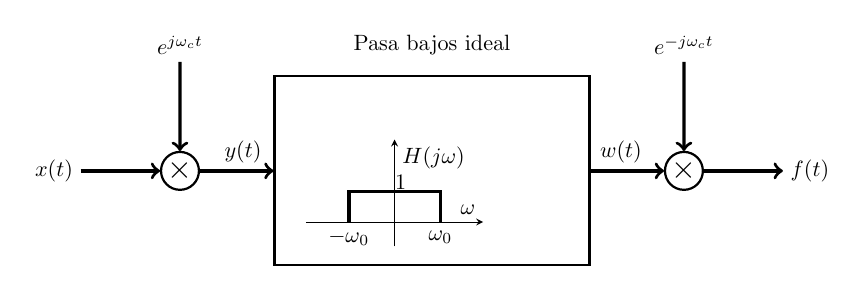
\begin{tikzpicture}[scale=0.8, transform shape]
    \node[rectangle, draw, thick, minimum height=3cm, minimum width=5cm] (hpb) at (0,0) {} ;
    \begin{axis}[
        x=0.04\textwidth,y=0.04\textwidth,
        axis y line=center,
        axis x line=middle,
        xlabel=$\omega$,ylabel={ $H(j\omega)$},
        xmin=-2.9,xmax=2.9,
        ymin=-0.8,ymax=2.7,
        ticks=none,
        at={(-2cm,-1.2cm)}
        ]
        \addplot[
        black,
        ultra thick
        ] coordinates {
            (-1.5,0) (-1.5,1) (1.5,1) (1.5,0)
        } ;
        \node at (-1.5,-.5) {$-\omega_0$};
        \node at (1.5,-.5) {$\omega_0$};
        \node at (0.2,1.3) {1} ;
    \end{axis} 
    \node[yshift=2cm] (hpb_label) at (hpb) {Pasa bajos ideal} ;

    \node[circle,draw,thick,inner sep=0.03cm, xshift=4cm] (mult_after) at (hpb) {\Large $\times$} ;
    \node[circle,draw,thick,inner sep=0.03cm, xshift=-4cm] (mult_before) at (hpb) {\Large $\times$} ;
    \node[yshift=2cm] (exp_after) at (mult_after) {$e^{-j\omega_c t}$} ;
    \node[yshift=2cm] (exp_before) at (mult_before) {$e^{j\omega_c t}$} ;
    \node[xshift=-2cm] (x_t) at (mult_before) {$x(t)$} ;
    \node[xshift=1cm,yshift=0.3cm] (y_t) at (mult_before) {$y(t)$} ;
    \node[xshift=2cm] (f_t) at (mult_after) {$f(t)$} ;
    \node[xshift=-1cm,yshift=0.3cm] (w_t) at (mult_after) {$w(t)$} ;

    \draw[->, very thick] (x_t.east) -- (mult_before.west) ;
    \draw[->, very thick] (mult_before.east) -- (hpb.west) ;
    \draw[->, very thick] (hpb.east) -- (mult_after.west) ;
    \draw[->, very thick] (mult_after.east) -- (f_t.west) ;
    \draw[->, very thick] (exp_before.south) -- (mult_before.north);
    \draw[->, very thick] (exp_after.south) -- (mult_after.north);
\end{tikzpicture}}
    \end{center}
\end{ejercicio}